\documentclass[a4paper,12pt]{article}

\usepackage[spanish]{babel}
\usepackage[utf8]{inputenc}
\usepackage[T1]{fontenc}
\usepackage[utf8]{inputenc}
\usepackage{makeidx}
\usepackage{graphicx}
\usepackage{lmodern}
\usepackage{kpfonts}
\usepackage[left=2cm,right=2cm,top=2cm,bottom=2cm]{geometry}
\usepackage{amsmath,amsfonts,amssymb}
\usepackage{setspace}

\title{Tarea 1}
\author{Junior Miguel Lara Torres}
\date{today}

\graphicspath {{C:/Users/JuniorLara/Desktop/TexMaker_Files/}}
\begin{document}

\begin{center}
\par 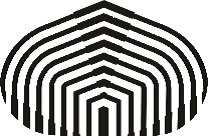
\includegraphics[scale=1]{USB} \par
Universidad Simon Bolivar \\ Curso: CI2613 / Algoritmos y Estructuras III \\ Trimestre: Septiembre-Diciembre, 2022 \\ Profesor: Wilmer Bandres \\ Estudiante: Junior Miguel Lara Torres - Carnet: 17-10303 \\
\end{center}

\begin{center}
Tarea 1
\end{center}

\textbf{1. Conceptos (3 pts)} \\

$ ~~~~~~ $ • Defina un grafo no dirigido \\

Sea un grafo G = (V,E), se dice que G es un grafo no dirigido formado por $V = \{n_1, n_2, ..., n_k\}$ si el conjunto E se expresa de la forma $E = \{ \{n_1,n_2\}, \{n_2,n_3\}, ..., \{n_i,n_j\} \}$ con $1\leq i, j\leq k \land i \neq j$. \\

$ ~~~~~~ $ • Defina un grafo dirigido \\

Sea un grafo G = (V,E), se dice que G es un grafo dirigido formado por $V = \{n_1, n_2, ..., n_k\}$ si el conjunto E se expresa de la forma $E = \{ (n_1,n_2), (n_2,n_3), ..., (n_i,n_j) \}$ con $1\leq i, j\leq k \land i \neq j$. Cabe destacar que el par $(n_1,n_2) \neq (n_2,n_1)$. \\

$ ~~~~~~ $ • Defina el grado de un nodo \\

Sea un grafo G = (V,E) y $x \in V$, se define $\delta(x) = \{\{x,y\} : \{x,y\} \in E \text{ para algun } y\} $. Por tanto, se define grado de un nodo x como $|\delta(x)|$. \\

$ ~~~~~~ $ • ¿Qué significa que un nodo sea adyacente a otro?, intente describirlo formalmente \\

Sea un grafo G = (V,E), se tiene un arco $e \in E$, decimos que $x,y \in V$ son adyacentes si $x \in e \land y \in e$. \\

$ ~~~~~~ $ • ¿Qué significa que un nodo es incidente a una arista?, intente describirlo formalmente \\

Sea un grafo G = (V,E), se define nodo incidente cuando un arco $\{x,y\} = e \in E$, el nodo x es incidente a $e$ si $x \in e$. \\

$ ~~~~~~ $ • Defina: \\

$ ~~~~~~ $ – Grafo completo: \\

Sea un grafo G = (V,E) se dice que G es completo si $\forall x,y \in V \implies \{x,y\} \in E$. Se denota por $G = (V, (V \times V) \setminus \{\{x, x \}: \forall x \in V\})$. Se denota $K_n$ al grafo completo de n nodos. \\

$ ~~~~~~ $ – Grafo inducido: \\

Sea un grafo G = (V,E), se toma $V' \subseteq V$ y se define grafo inducido como $G'$ = (V',E') donde E' es el conjunto de arcos que conforman los nodos pertenecientes a V'. \\

$ ~~~~~~ $ – Clique de un grafo: \\

Sea un G = (V,E), $V' \subseteq V$ y $G'$ = (V',E') un grafo inducido. Se dice que $G'$ es un clique si $G'$ es completo. \\

$ ~~~~~~ $ – Grafo bipartito: \\

Sea un grafo $G = (V \dot{\cup} W, E)$ donde $V \dot{\cup} W$ es la unión de conjuntos disjuntos ($V \cap W \neq \emptyset$). Se dice que G es bipartito si \par 

\begin{center}
$\left\{\begin{matrix}
\forall x, y \in V: \not \exists \{x,y\} \in E \\
\forall x, y \in W: \not \exists \{x,y\} \in E
\end{matrix}\right. $ \\
\end{center}

$ ~~~~~~ $ – Grafo Euleriano: \\

Es un grafo conexo de la forma G = (V,E) tal que $\forall v \in V : |\delta(v)|\equiv_2 0$ \\

$ ~~~~~~ $ – Grafo Hamiltoniano: \\

Se dice que un grafo Hamiltoniano es aquel que admite un camino Hamiltoniano. Un camino hamiltoniano es un camino simple $P$ para cualquier G = (V,E), dirigido o no, cuya longitud es $L(P) = |V| - 1$. Es decir, es un camino simple que pasa por todos los nodos del grafo.

Nota: Wikipedia dice que: 

Se enuncia el Teorema de Dirac:
\begin{center}
"Sea G = (V,E) un grafo conexo con $|V| \geq 3$. Si $|\delta(v)|\geq |V|/2$ para todo $v \in V$, entonces G es Hamiltoniano."
\end{center}

$ ~~~~~~ $ – Grafo regular: \\

Sea un grafo G = (V,E) se dice que es regular si $\forall x \in V \implies |\delta(x)| = k$ con k constante. \\

$ ~~~~~~ $ – Número cromático de un grafo: \\

Seae un grafo G se define número cromático $\chi(G)$ como el mínimo número de colores con el que se puede colorear G sin que dos nodos adyacentes tengan el mismo color. \\

$ ~~~~~~ $ – Grafo k-coloreable: \\

Sea G = (V,E) un grafo tal que es posible colorearlo con exactamente k colores, entonces se dice que G es k-coloreable. \\ $~~ \\ ~~ \\ ~~ \\ $

$ ~~~~~~ $ – Ciclo de un grafo: \\

Sea G = (V,E) un grafo, se define como ciclo a un camino $C = \langle n_1,n_2, ..., n_k, n_1\rangle$ que empieza y termina en el mismo nodo, solo se repite 1 nodo y es el "nodo inicial". \\

$ ~~~~~~ $ – Circuito de un grafo: \\

Sea G = (V,E) un grafo dirigido, se define como ciclo a un camino $C = \langle n_1,n_2, ..., n_k, n_1\rangle$ que empieza y termina en el mismo nodo, solo se repite 1 nodo y es el "nodo inicial". \\

$ ~~~~~~ $ – Alcanzabilidad en un grafo: \\

Sea G = (V,E) dirigido o no, se tiene $a,b \in V$ decimos que $a$ alcanza a $b$ si existe un camino C desde $a$ hasta $b$. \\

$ ~~~~~~ $ – Dado un grafo $G = (V,E)$, qué representa $E^k$: \\

$E^k$ representa el conjunto, de conjuntos en caso no dirigido o de pares ordenados en caso dirigido, tal que para los $\{x,y\} \in E^k$ establece una relación de alcanzabilidad en k pasos. Es decir, existe un camino entre $x$ e $y$ de tamaño k. \\

\textbf{2. Aplicación de los Conceptos (7 pts)} \\

$ ~~~~~~ $ • Dé ejemplos de un grafo Euleriano y uno Hamiltoniano\\

Ej. Grafo Euleriano:  \\

\begin{center}
\par 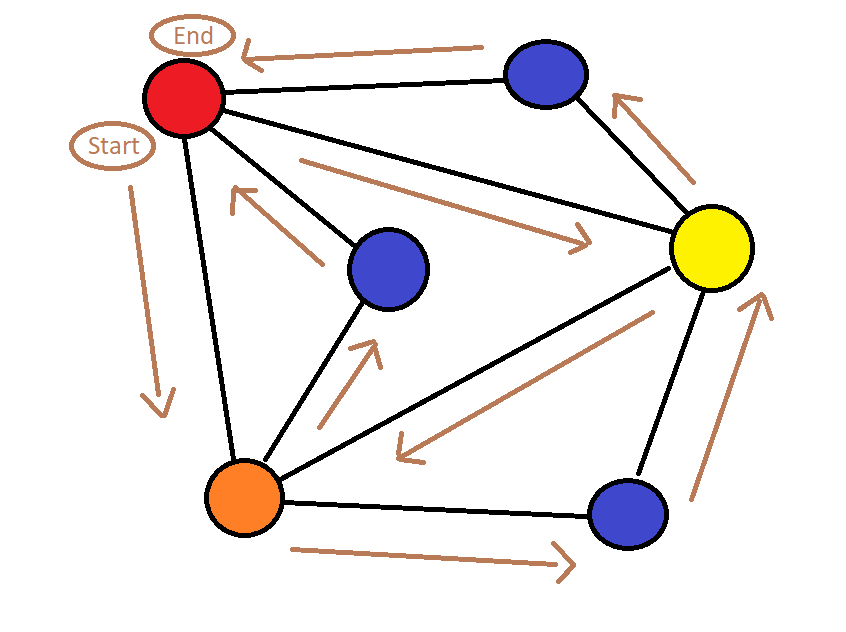
\includegraphics[scale=0.8]{grafoeuleriano} \par
\end{center} 

$ \\ ~~ \\ ~~ $ Ej. Grafo Hamiltoniano: \\

\begin{center}
\par 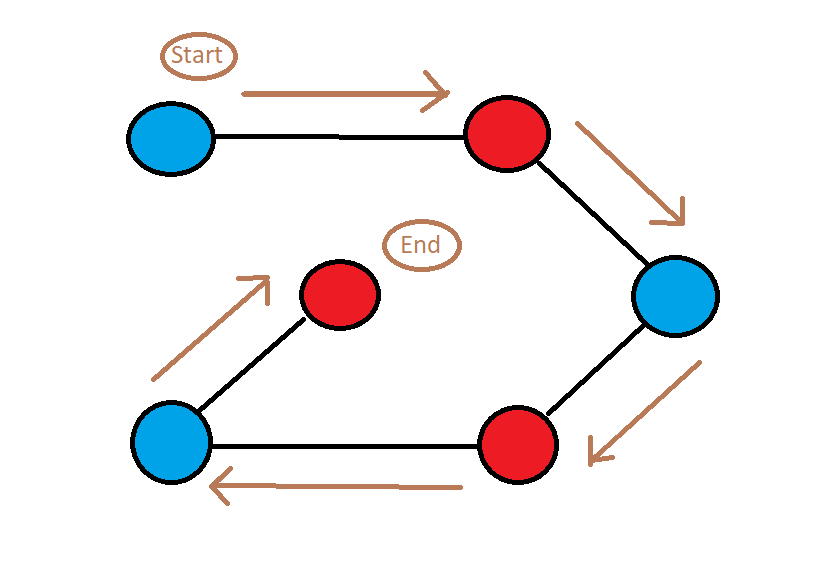
\includegraphics[scale=0.8]{grafohamiltoniano} \par
\end{center}

$ ~~~~~~ $ • Dé ejemplo de un grafo 2-regular \\

\begin{center}
\par 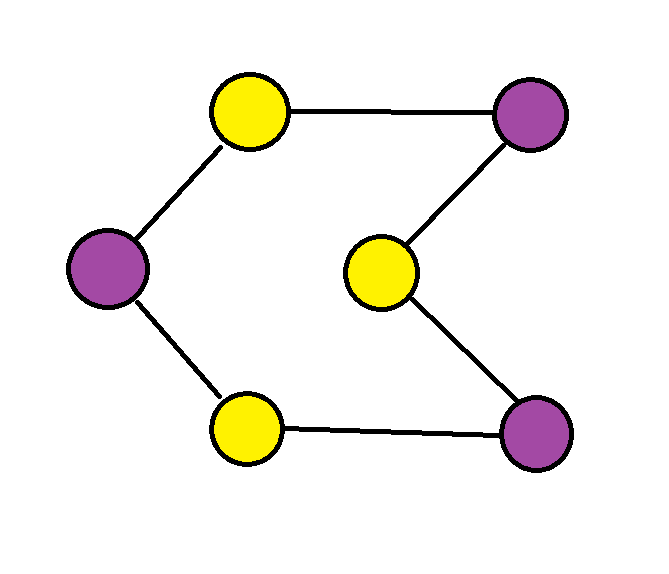
\includegraphics[scale=0.8]{graforegular} \par
\end{center}

$ ~~ \\ ~~ \\ ~~ \\ ~~ \\ ~~ \\ $ 
$ ~~~~~~ $ • Dé un algoritmo (no importa su complejidad) para colorear un grafo con k colores \\
\\
bool K-coloreable(G=(V,E), int k) $\{$ \\
$~~~~~~~~$ list ListColors[k];$~~~~~~~~~~~~~~~~~~~$/Lista de k colores(index-1)/ \\
$~~~~~~~~$ Queue Cola $\leftarrow$ $\emptyset$;$~~~~~~~~~~~~~~~~~~~$/Cola vacia/ \\
\\
$~~~~~~~~$ Si $k > |V|$ hacer $\{$ \\
$~~~~~~~~~~~~~~~~$ print("No es posible colorear con \{k\} > \{|V|\}")\\
$~~~~~~~~~~~~~~~~$ return 0;\\
$~~~~~~~~$ $\}$\\
\\
$~~~~~~~~$ /La etiqueta 0 indica Nunca visitado, la etiqueta 1 indica Ya visitado./\\
$~~~~~~~~$ Para $v \in V$ hacer $\{$ \\
$~~~~~~~~~~~~~~~~$ v.etiqueta = 0;\\
$~~~~~~~~$ $\}$\\
\\
$~~~~~~~~$ /Buscamos un nodo con el grado menor a la cantidad de colores para iniciar./\\
$~~~~~~~~$ nodo = RandomNode(V);\\
$~~~~~~~~$ Para $v \in V$ hacer $\{$ \\
$~~~~~~~~~~~~~~~~$ Si $|G.adyacencias[v]| < k$ hacer $\{$ \\
$~~~~~~~~~~~~~~~~~~~~~~~~$ nodo = v;\\
$~~~~~~~~~~~~~~~~~~~~~~~~$ break;\\
$~~~~~~~~~~~~~~~~$ $\}$\\
$~~~~~~~~$ $\}$\\
\\
$~~~~~~~~$ nodo.etiqueta = 1;\\
$~~~~~~~~$ nodo.color = ListColors[1];\\
$~~~~~~~~$ Cola.agregar(nodo);\\
$~~~~~~~~$ int ColoresUsados = 1;\\
$~~~~~~~~$ int NodosVisitados = 1;\\
\\
$~~~~~~~~$/Sacamos un nodo, trabajamos con sus adyacentes. Se pitan los adyacentes en\\ $~~~~~~~~$ funciones de los colores usados en los adyacentes. Es decir, adyacentes de los\\ $~~~~~~~~$ adyacentes que sean visitados (etiqueta 1) serán esos colores los eliminados \\ $~~~~~~~~$ en la lista de colores aux./\\
$~~~~~~~~$ Mientras $Cola \neq \emptyset$ hacer $\{$ \\
$~~~~~~~~~~~~~~~~$ int m $\leftarrow$ Cola.sacar();\\
$~~~~~~~~~~~~~~~~$ list aux = ListColors;\\
\\
$~~~~~~~~~~~~~~~~$ Para $v \in G.adyacentes[m]$ hacer $\{$ \\
$~~~~~~~~~~~~~~~~~~~~~~~~$ Si $v.etiqueta == 0$ hacer $\{$ \\
$~~~~~~~~~~~~~~~~~~~~~~~~~~~~~~~~$ v.etiqueta = 1;\\
$~~~~~~~~~~~~~~~~~~~~~~~~~~~~~~~~$ NodosVisitados++;\\
$~~~~~~~~~~~~~~~~~~~~~~~~~~~~~~~~$ Si $ColoresUsados < k$ hacer $\{$ \\
$~~~~~~~~~~~~~~~~~~~~~~~~~~~~~~~~~~~~~~~~$ ColoresUsados++;\\
$~~~~~~~~~~~~~~~~~~~~~~~~~~~~~~~~~~~~~~~~$ v.color = ListColors[ColoresUsados]; \\
$~~~~~~~~~~~~~~~~~~~~~~~~~~~~~~~~$ $\}$ Si no hacer $\{$ \\
$~~~~~~~~~~~~~~~~~~~~~~~~~~~~~~~~~~~~~~~~$ Para $t \in G.adyacentes[v]$ hacer $\{$ \\	
$~~~~~~~~~~~~~~~~~~~~~~~~~~~~~~~~~~~~~~~~~~~~~~$ Si $t.etiqueta == 1$ hacer $\{$\\
$~~~~~~~~~~~~~~~~~~~~~~~~~~~~~~~~~~~~~~~~~~~~~~~~~~~~$ aux[t.color] = -1;\\
$~~~~~~~~~~~~~~~~~~~~~~~~~~~~~~~~~~~~~~~~~~~~~~$ $\}$\\
$~~~~~~~~~~~~~~~~~~~~~~~~~~~~~~~~~~~~~~~~$ $\}$\\
$~~~~~~~~~~~~~~~~~~~~~~~~~~~~~~~~~~~~~~~~$ c = 1;\\
$~~~~~~~~~~~~~~~~~~~~~~~~~~~~~~~~~~~~~~~~$ Mientras $c \leq k$ hacer $\{$ \\
$~~~~~~~~~~~~~~~~~~~~~~~~~~~~~~~~~~~~~~~~~~~~~~~~$ Si $aux[c] \neq -1$ hacer $\{$ \\
$~~~~~~~~~~~~~~~~~~~~~~~~~~~~~~~~~~~~~~~~~~~~~~~~~~~~~~~~$ v.color = ListColors[c];	\\
$~~~~~~~~~~~~~~~~~~~~~~~~~~~~~~~~~~~~~~~~~~~~~~~~~~~~~~~~$ break;\\
$~~~~~~~~~~~~~~~~~~~~~~~~~~~~~~~~~~~~~~~~~~~~~~~~$ $\}$\\
$~~~~~~~~~~~~~~~~~~~~~~~~~~~~~~~~~~~~~~~~~~~~~~~~$ c++;\\
$~~~~~~~~~~~~~~~~~~~~~~~~~~~~~~~~~~~~~~~~~~~~~~~~$ Si $c > k$ hacer $\{$ \\
$~~~~~~~~~~~~~~~~~~~~~~~~~~~~~~~~~~~~~~~~~~~~~~~~~~~~~~~~$ print ("No {k}-Coloreable.");\\
$~~~~~~~~~~~~~~~~~~~~~~~~~~~~~~~~~~~~~~~~~~~~~~~~~~~~~~~~$ return 0; \\	
$~~~~~~~~~~~~~~~~~~~~~~~~~~~~~~~~~~~~~~~~~~~~~~~~$ $\}$\\
$~~~~~~~~~~~~~~~~~~~~~~~~~~~~~~~~~~~~~~~~$ $\}$	\\
$~~~~~~~~~~~~~~~~~~~~~~~~~~~~~~~~$ $\}$\\
$~~~~~~~~~~~~~~~~~~~~~~~~~~~~~~~~$ Cola.agregar(v);\\
$~~~~~~~~~~~~~~~~~~~~~~~~$ $\}$\\
$~~~~~~~~~~~~~~~~$ $\}$\\
$~~~~~~~~~~~~~~~~$ /En caso de haber en el grafo dos o mas conjunto de nodos que\\
$~~~~~~~~~~~~~~~~$ no se conectan entre si, entonces nos aseguramos se recorrer o\\ 
$~~~~~~~~~~~~~~~~$ visitar todos los nodos del grafo./ \\
$~~~~~~~~~~~~~~~~$ Si $Cola == \emptyset \land NodosVisitados < |V|$ hacer $\{$ \\
$~~~~~~~~~~~~~~~~~~~~~~~~$ Para $v \in V$ hacer $\{$ \\
$~~~~~~~~~~~~~~~~~~~~~~~~~~~~~~~~$ Si $v.etiqueta == 0$ $\{$ \\
$~~~~~~~~~~~~~~~~~~~~~~~~~~~~~~~~~~~~~~~~$ v.etiqueta = 1;\\
$~~~~~~~~~~~~~~~~~~~~~~~~~~~~~~~~~~~~~~~~$ Si $ColoresUsados < k$ hacer $\{$ \\
$~~~~~~~~~~~~~~~~~~~~~~~~~~~~~~~~~~~~~~~~~~~~~~~~$ ColoresUsados++; \\
$~~~~~~~~~~~~~~~~~~~~~~~~~~~~~~~~~~~~~~~~~~~~~~~~$ v.color = ListColors[ColoresUsados];\\
$~~~~~~~~~~~~~~~~~~~~~~~~~~~~~~~~~~~~~~~~$ $\}$ Si no hacer $\{$ \\
$~~~~~~~~~~~~~~~~~~~~~~~~~~~~~~~~~~~~~~~~~~~~~~~~$ v.color = ListColors[1];\\
$~~~~~~~~~~~~~~~~~~~~~~~~~~~~~~~~~~~~~~~~$ $\}$ \\
$~~~~~~~~~~~~~~~~~~~~~~~~~~~~~~~~~~~~~~~~$ NodosVisitados++;\\
$~~~~~~~~~~~~~~~~~~~~~~~~~~~~~~~~~~~~~~~~$ Cola.agregar(v);\\
$~~~~~~~~~~~~~~~~~~~~~~~~~~~~~~~~~~~~~~~~$ break;\\
$~~~~~~~~~~~~~~~~~~~~~~~~~~~~~~~~$ $\}$ \\
$~~~~~~~~~~~~~~~~~~~~~~~~$ $\}$ \\
$~~~~~~~~~~~~~~~~$ $\}$\\
$~~~~~~~~$ $\}$\\
$~~~~~~~~$ Si $ColoresUsados == k$ hacer $\{$ \\
$~~~~~~~~~~~~~~~~$ print ("Se coloreo con {k} colores.");\\
$~~~~~~~~~~~~~~~~$ return 1;\\
$~~~~~~~~$ $\}$ Si no hacer $\{$ \\
$~~~~~~~~~~~~~~~~$ print ("No {k}-Coloreable.");\\
$~~~~~~~~~~~~~~~~$ return 0;\\
$~~~~~~~~$ $\}$\\
$\}$\\
\\ Se usa la noción de cola para ir llevando un orden en el recorrido del grado. Una vez se elija un nodo, se trabaje con él, los nodos adyacentes se agregan a la cola en orden en que fueron visitados, esto permite recorrer el grafo he ir pintando en función de los adyacentes. \\

$ ~~~~~~ $ • Dé un algoritmo para determinar si un grafo es bipartito o no \\
\\
bool G-Bipartito(G=(V,E)) $\{$ \\
$~~~~~~~~$ / Por teorema si un grafo es 2-coloreable entonces es bipartito./ \\
$~~~~~~~~$ Si $K-coloreable(G=(V,E), 2)$ hacer $\{$\\
$~~~~~~~~~~~~~~~~$ print('Es Bipartito');\\
$~~~~~~~~~~~~~~~~$ return 1;\\
$~~~~~~~~$ $\}$ Si no hacer $\{$\\
$~~~~~~~~~~~~~~~~$ print('No es Bipartito');\\
$~~~~~~~~~~~~~~~~$ return 0;\\
$~~~~~~~~$ $\}$\\
$\}$ \\

$ ~~~~~~ $ • Asuma que usted ha construido un algoritmo que indica si un grafo tiene un clique de tamaño k. Construya un algoritmo que indique si un grafo no es k'-coloreable (estando 100$\%$ seguro) o retorne ”No sé” \\
\\
Digamos que la función G-Clique recibe un grafo G=(V,E) y retorna el tamaño del clique encontrado. Retorna 0 en caso de no encontrar un clique.\\
\\
bool NOK-coloreable(G=(V,E), k) $\{$ \\
$~~~~~~~~$ /Por def. de Clique, si es de tamaño k quiere decir que el grafo inducido por \\
$~~~~~~~~$ G[V'] es completo y por def. de grafo completo $\forall x,y \in V' \implies \{x,y\} \in E$, por tanto se \\
$~~~~~~~~$ necesitan k colores para pintar ese clique nada mas./\\
$~~~~~~~~$ \\
$~~~~~~~~$ Si $(k < G-Clique(G=(V,E))) \vee (k > |V|)$ hacer $\{$ \\
$~~~~~~~~~~~~~~~~$ print("No es posible colorear")\\
$~~~~~~~~~~~~~~~~$ return 1;\\
$~~~~~~~~$ $\}$ Si no hacer $\{$\\
$~~~~~~~~~~~~~~~~$ print("No sé")\\
$~~~~~~~~~~~~~~~~$ return 0;\\
$~~~~~~~~$ $\}$ \\
$\}$ \\

Se me ocurren dos casos en que puedo afirmar no es k coloreable. Cuando se afirma un clique de tamaño k se requiera k colores mínimo, entonces usar un k' < k no es posible. La otra es cuando el k pedido es mayor al numero de nodos. Esta el caso borde de k = 0, pero asumiremos que al menos k > 0 y un numero entero.\\

\begin{center}
\par 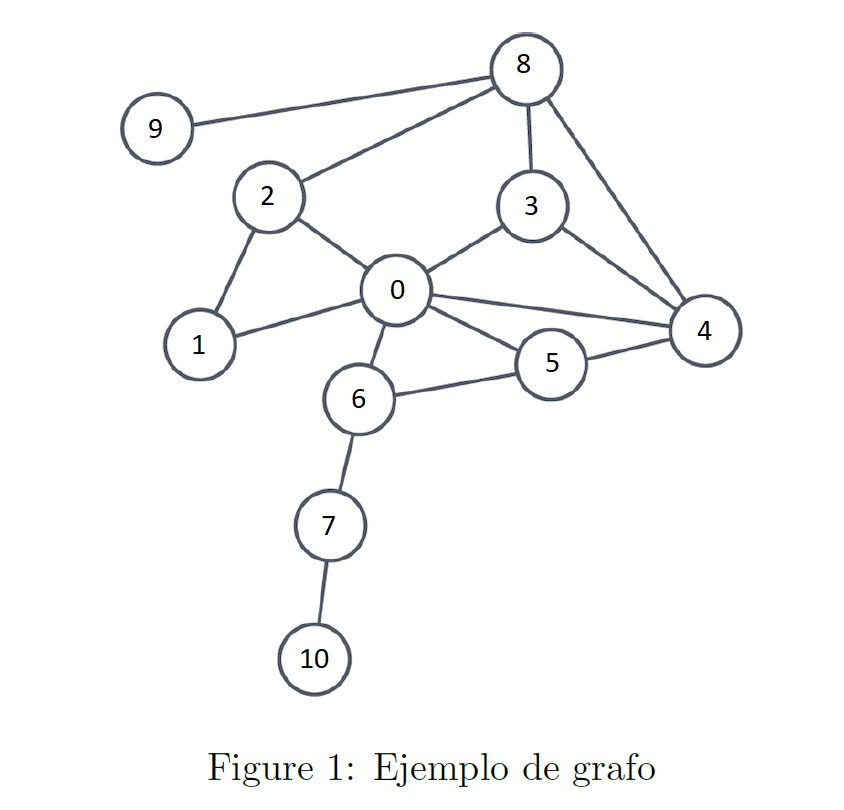
\includegraphics[scale=0.8]{f1} \par
\end{center}

$ ~~~~~~ $ • De la representación del siguiente grafo mediante lista de adyacencias y matriz de adyacencias del grafo en la figura 1 \\

La lista de adyacencia respectiva es:\\

Nodos\\
$~~~\fbox{0}$ $\to$ $\fbox{1}$ $\to$ $\fbox{2}$ $\to$ $\fbox{3}$ $\to$ $\fbox{4}$ $\to$ $\fbox{5}$ $\to$ $\fbox{6} \dashv$ \\
$~~~\fbox{1}$ $\to$ $\fbox{0}$ $\to$ $\fbox{2} \dashv$ \\
$~~~\fbox{2}$ $\to$ $\fbox{0}$ $\to$ $\fbox{1}$ $\to$ $\fbox{8} \dashv$ \\
$~~~\fbox{3}$ $\to$ $\fbox{0}$ $\to$ $\fbox{4}$ $\to$ $\fbox{8} \dashv$ \\
$~~~\fbox{4}$ $\to$ $\fbox{0}$ $\to$ $\fbox{3}$ $\to$ $\fbox{5}$ $\to$ $\fbox{8} \dashv$ \\
$~~~\fbox{5}$ $\to$ $\fbox{0}$ $\to$ $\fbox{4}$ $\to$ $\fbox{6} \dashv$ \\
$~~~\fbox{6}$ $\to$ $\fbox{0}$ $\to$ $\fbox{5}$ $\to$ $\fbox{7} \dashv$ \\
$~~~\fbox{7}$ $\to$ $\fbox{6}$ $\to$ $\fbox{10} \dashv$ \\
$~~~\fbox{8}$ $\to$ $\fbox{2}$ $\to$ $\fbox{3}$ $\to$ $\fbox{4}$ $\to$ $\fbox{9} \dashv$ \\
$~~~\fbox{9}$ $\to$ $\fbox{8} \dashv$ \\
$~~~\fbox{10}$ $\to$ $\fbox{7} \dashv$\\

La matriz de adyacencia respectiva es:

\begin{center}
$\begin{pmatrix}
    0 & 1 & 1 & 1 & 1 & 1 & 1 & 0 & 0 & 0 ~~~ 0 \\
    1 & 0 & 1 & 0 & 0 & 0 & 0 & 0 & 0 & 0 ~~~ 0 \\
    1 & 1 & 0 & 0 & 0 & 0 & 0 & 0 & 1 & 0 ~~~ 0 \\
    1 & 0 & 0 & 0 & 1 & 0 & 0 & 0 & 1 & 0 ~~~ 0 \\
    1 & 0 & 0 & 1 & 0 & 1 & 0 & 0 & 1 & 0 ~~~ 0 \\
    1 & 0 & 0 & 0 & 1 & 0 & 1 & 0 & 0 & 0 ~~~ 0 \\
    1 & 0 & 0 & 0 & 0 & 1 & 0 & 1 & 0 & 0 ~~~ 0 \\
    0 & 0 & 0 & 0 & 0 & 0 & 1 & 0 & 0 & 0 ~~~ 1 \\
    0 & 0 & 1 & 1 & 1 & 0 & 0 & 0 & 0 & 1 ~~~ 0 \\
    0 & 0 & 0 & 0 & 0 & 0 & 0 & 0 & 1 & 0 ~~~ 0 \\
    0 & 0 & 0 & 0 & 0 & 0 & 0 & 1 & 0 & 0 ~~~ 0 \\
\end{pmatrix}$ 
\end{center}

$ ~~~~~~ $ * Diga que ventajas presenta la representación de un grafo mediante matriz de adyacencias y que desventajas presenta \\

Por parte de listas de adyacencias tenemos un punto a favor en el espacio/memoria utilizado dado que es memoria ajustada a los datos necesarios, a diferencia de las matrices se tiene mayor memoria pues ese 0 representado en matriz es información extra que no se refleja en las listas. 

El otro punto fuerte es la ventaja de las operaciones. El punto a favor se la llevan las matrices dado que las operaciones/algebra de grafos en su mayoría son constantes en tiempo, la única operaciones costosa es añadir un nodo dado que se debe reestructurar la matriz. Por otra parte, las listas de adyacencias tienen mas operaciones en funcion del numero de nodos que constantes. Sin embargo, al tomar vectores dinámicos junto con arreglos puede ser mas eficiente el uso de listas. \\

\textbf{3. Demostraciones (5 pts)} \par
Demuestre (o muestre un contraejemplo) de las siguiente proposiciones. \\

• Un grafo es 2-coloreable si y sólo si es bipartito \\

($\Rightarrow$) Si tenemos un grafo 2-coloreable entonces quiere decir que para todo nodo x tiene un color distinto al conjunto de todos los nodos adyacentes a x. Esta relación permite establecer que el conjunto de adyacentes de x contiene un color y los nodos que sobren contando a x tienen otro color. Entonces, hemos formado dos conjuntos disjuntos a nivel de color y por consiguiente tales que no se conectan entre ellos, pues de haber una arista entre un nodo adyacente a x y otro nodo también adyacente a x se formaría un ciclo lo que evita poder ser grafo 2-coloreable. Así, podemos dar pie a la definición de grafo bipartito. \\

($\Leftarrow$) Por definición de Bipartito se tiene que existe un conjunto V y W tales que son disjuntos ($V \cap W = \emptyset$) y que a su vez indican que entre los elementos del conjunto V no existe conexión alguna, los ismo pasa con W. Asi, podemos tener un numero cromático de 2, lo que afirma que el grafo es 2-coloreable. \\ 

• Si un grafo es k-coloreable entonces es también $(k + n)$ coloreable para $n \geq 1$ \\

Supongamos que tenemos un grafo con $|V|$ nodos. Decimos que es k coloreable, este $k \leq |V|$ pues en caso de $k > |V|$ seria un absurdo pues hay mas colores que nodos. Ahora bien, se dice que si para $k \leq |V|$ el grafo es coloreable, tendremos que en algún punto para $n \geq 1$ ocurre que $k+n > |V|$ por tanto es absurdo tener que para todo k+n con $n \geq 1$ es siempre coloreable. 

PD: Pensaba hacer un contraejemplo de dibujos, pero preferí tomar la vía de demostración "formal/escrita" para practicar.\\

• Si un grafo tiene un clique de tamaño k entonces el grafo es $(k-1)$-coloreable \\

Por definición en un grafo G =(V,E) al tomar un $V' \subseteq V$ se dice que el grafo inducido $G[V']$ es un clique si $G[V']$ es un grafo completo. Entonces, es sabido que todo conjunto es subconjunto de si mismo ($V \subseteq V$). Por tanto si al tomar $V' = V$ es decir que el grafo original es un clique de tamaño k ($]V]=k$)y por definición de grafo completo todo par de nodos x e y implican que el par $\{x,e\} \in E$ y por definicion de coloreabilidad en un grafo completo se deben usar $|V|$ colores, por consiguiente no es posible pintar con $|V|-1 = k-1$ colores.
 
\end{document}
